\begin{frame}
    \frametitle{Herleitung der Fourier Transformation} 

    \begin{align*}
        (\mathcal{F} g)(f)=\int_{-\infty}^{\infty}{g(t)\cdot e^{-i2\pi f t}\ dt}
    \end{align*}
\end{frame}

\begin{frame}
    \frametitle{Herleitung der Fourier Transformation}
    \framesubtitle{Eulersche Formel}

    \hspace{-100px}
    \begin{columns}[c]
        \begin{column}{200px}
        \begin{align*}
        e^{i\varphi}=\cos{\varphi}+i\sin{\varphi}
    \end{align*}
\end{column}
\hspace*{-60px}
\begin{column}{100px}
    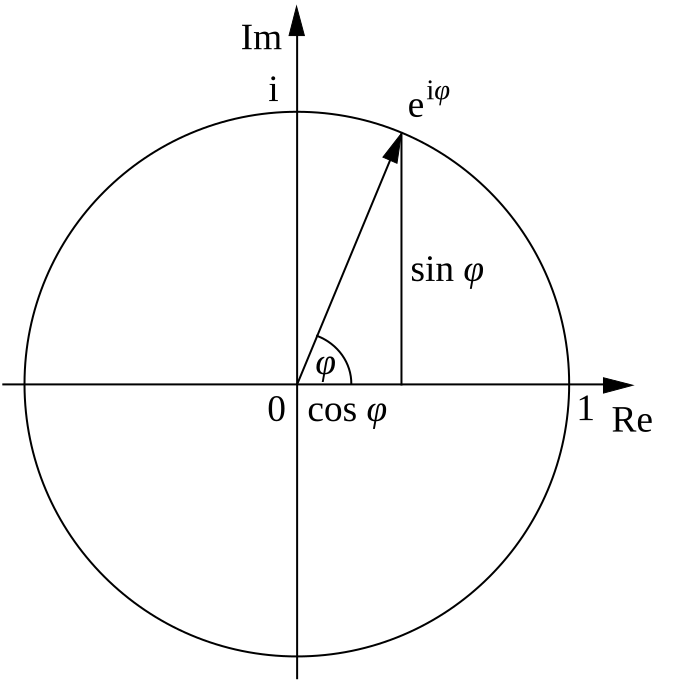
\includegraphics[width=100px]{images/02-deriving-fourier-euler.png}
\end{column}
    \end{columns}
\end{frame}

\begin{frame}
    \frametitle{Herleitung der Fourier Transformation}
    \framesubtitle{Eulersche Formel}

    \hspace{-100px}
    \begin{columns}[c]
        \begin{column}{200px}
        \begin{align*}
        e^{i\varphi}=\cos{\varphi}+i\sin{\varphi}
    \end{align*}
\end{column}
\hspace*{-60px}
\begin{column}{100px}
    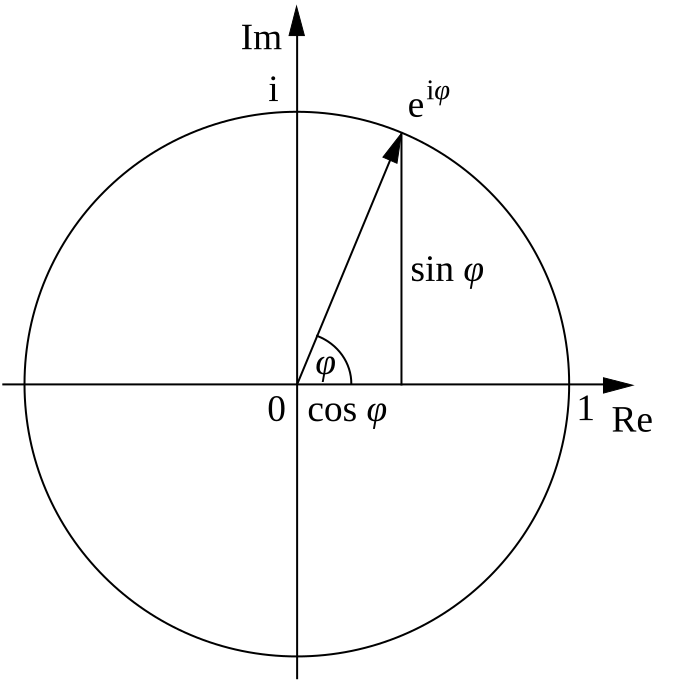
\includegraphics[width=100px]{images/02-deriving-fourier-euler.png}
\end{column}
    \end{columns}
    \vspace{20px}
    Rotieren in der komplexen Ebene mit Frequenz $f$: 
    \begin{align*}
        \varphi&=\omega t=2\pi ft \\
        c(t)&=e^{-i\varphi}\\
            &=e^{-i2\pi f t}
    \end{align*}
\end{frame}

\begin{frame}
    \frametitle{Herleitung der Fourier Transformation}
    \framesubtitle{Rotieren des Signals}

    Signal  $g(t)$ um einen Punkt in der komplexen Ebene rotieren:
    \begin{align*}
        g_c(t, f)=g(t)\cdot e^{-i2\pi f t}
    \end{align*}
    \begin{center}
        \begin{columns}[c]
    \begin{column}{100px}
        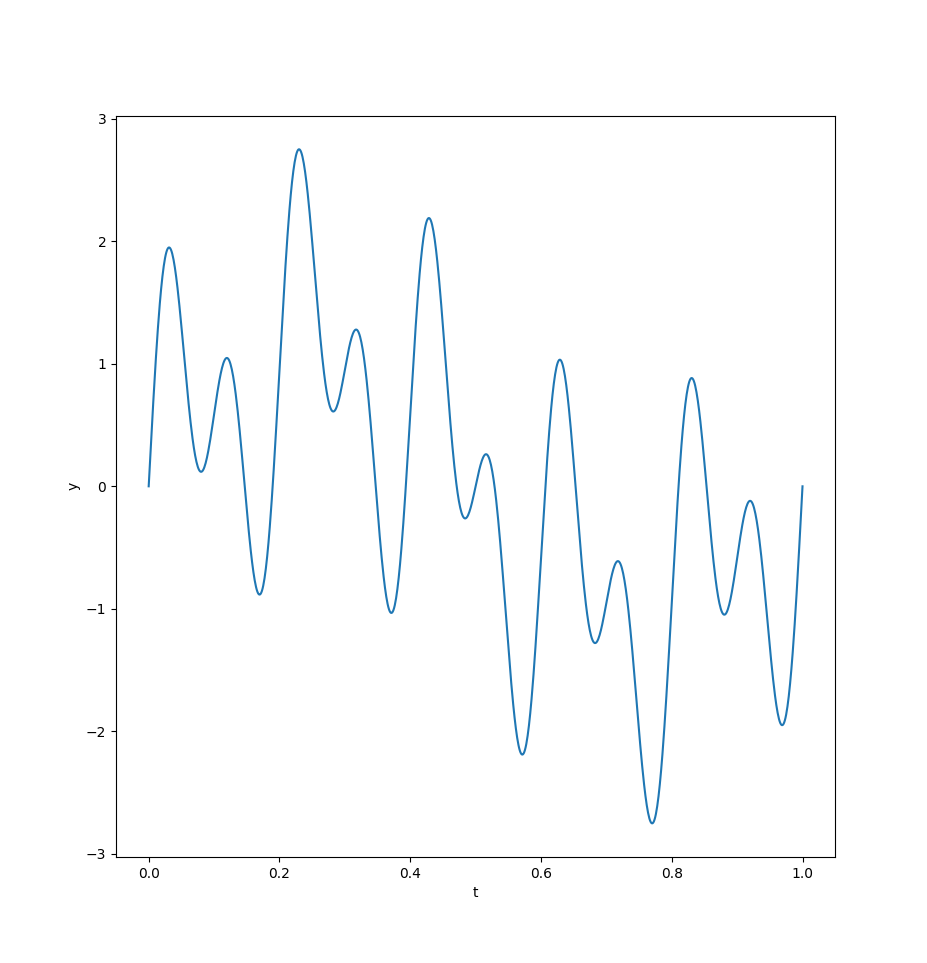
\includegraphics[width=100px]{images/01-what-is-fourier-signal.png}
    \end{column}
    \hspace*{-45px}
    \begin{column}{10px}
        $\overset{\scriptscriptstyle{f=10Hz}}{\parbox{1.1cm}{\rightarrowfill}}$
    \end{column}
    \hspace*{-20px}
    \begin{column}{100px}
        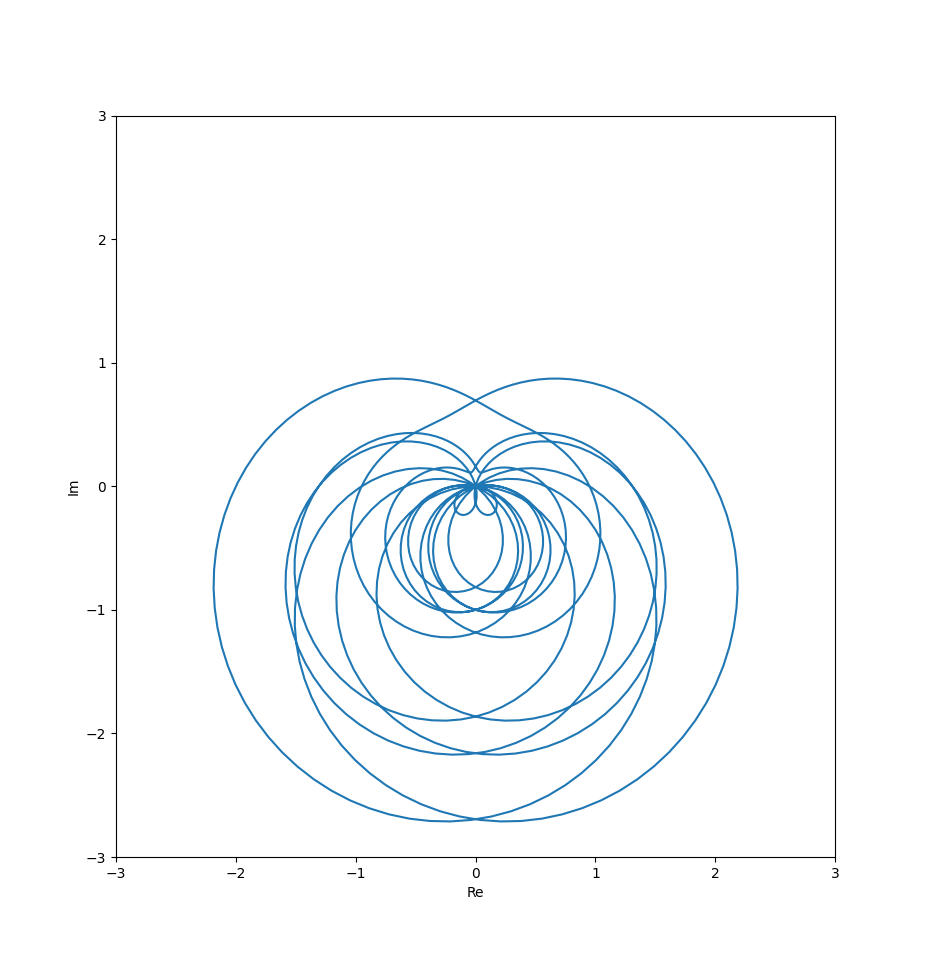
\includegraphics[width=100px]{images/02-deriving-fourier_wrapped_signal.png}
    \end{column}
    \end{columns}
    \end{center}
\end{frame}

\begin{frame}
    \frametitle{Herleitung der Fourier Transformation}
    \framesubtitle{Finden des Durchschnittswertes}
    Durchschnittlichen Wert von $f_c$ finden:
    \begin{align*}
    \frac{1}{N}\cdot \sum_{i=0}^{N}{g(t_i)\cdot e^{-i2\pi f t_i}}
    \end{align*}
    \begin{center}
    $\downarrow$ 
\end{center}
    \begin{align*}
        \frac{1}{t_2-t_1}\cdot \int_{t_1}^{t_2}{g(t)\cdot e^{-i2\pi f t}\ dt}
    \end{align*}
    \begin{itemize}
        \item[?]Entfernen des $\frac{1}{t_2-t_1}$ Terms 
    \end{itemize}
\end{frame}

\begin{frame}
    \frametitle{Herleitung der Fourier Transformation}
    \framesubtitle{Finden des Durchschnittswertes}
    Durchschnittlichen Wert von $f_c$ finden:
    \begin{align*}
        \frac{1}{t_2-t_1}\cdot \int_{t_1}^{t_2}{g(t)\cdot e^{-i2\pi f t}\ dt}
    \end{align*}
    \frametitle{Herleitung der Fourier Transformation}
    Entfernen des $\frac{1}{t_2-t_1}$ Terms:
    \begin{align*}
    \int_{t_1}^{t_2}{g(t)\cdot e^{-i2\pi f t}\ dt}
    \end{align*}
    \begin{itemize}
        \item Wenn eine Frequenz lange im Signal auftaucht, wird der Peak höher
    \end{itemize}
\end{frame}

\begin{frame}
    \frametitle{Herleitung der Fourier Transformation}
    Erweitern der Integrationsgrenzen:
    \begin{align*}
        \int_{-\infty}^{\infty}{g(t)\cdot e^{-i2\pi f t}\ dt}=(\mathcal{F}g)(f)
    \end{align*}

    \vspace{10px}
    \begin{tcolorbox}[colback=red!5!white,colframe=red!75!black,title=Wichtig]
        $(\mathcal{F} g):\mathbb{R}\rightarrow\mathbb{C}$ ist die komplexwertige Fourier Transformation\newline
        $\abs{(\mathcal{F} g)(f)}\ $ beschreibt die Anwesenheit von Frequenz $f$\newline
         $\angle (\mathcal{F} g)(f)\ $ ist die Phasenverschiebung von Frequenz $f$
    \end{tcolorbox}
\end{frame}
